\documentclass[11pt,a4paper]{article}

\usepackage[utf8]{inputenc}
\usepackage[margin=1in]{geometry}
\usepackage{amsmath}
\usepackage{amssymb}
\usepackage{amsfonts}
\usepackage{booktabs}
\usepackage{microtype}
\usepackage{pgfplots}
\pgfplotsset{compat=1.18}
\usepackage[numbers]{natbib}
\usepackage[hidelinks]{hyperref}

\hypersetup{
    pdftitle={Transplanting genes between effective-size compartments},
}

\newcommand{\Ne}{N_{e}}
\newcommand{\NA}{N_{\mathrm{A}}}
\newcommand{\NX}{N_{\mathrm{X}}}

\title{\textbf{Transplanting genes between effective-size compartments:\\ a within-genome probe of how linked selection scales}}
\author{\textbf{Daniel Ortiz-Barrientos}}
\date{\today}

\begin{document}

\maketitle

\begin{abstract}
\noindent Lewontin's paradox is a statement about \emph{scaling}: neutral diversity rises with population size far more shallowly than neutrality allows. Two mechanisms of linked selection sit behind that compression, and they scale oppositely with effective size---background selection lowers diversity by a factor that does not depend on population size, while genetic draft removes diversity ever more efficiently as population size grows. The cross-species axis that exposes this compression also confounds it, because population size travels through the data alongside mutation rate, generation time, recombination landscape, and demographic history. This essay develops a narrower and cleaner question. Within a single genome, inheritance compartments differ in effective size by known ratios, and a sequence relocated between them by retrotransposition or duplicative traffic is the same sequence observed in two effective-size environments. I show that the ratio of polymorphism to divergence, taken between two compartments of one genome, divides out both the mutation rate and the divergence time exactly, leaving the product of effective size and the linked-selection reduction. Under background selection this ratio equals the neutral effective-size ratio; under draft it exceeds it. That single inequality is the test. The effective-size lever inside a genome is small---at most fourfold---and it is entangled with selection-efficacy differences such as faster-X evolution, so a single contrast cannot carry the inference. I therefore nest the within-genome contrast inside the cross-species axis and ask whether the compartment ratio's departure from neutral expectation \emph{grows with species size}, which is the draft prediction stated one level up and stripped of the species-invariant confounds. I set out the theory, four progressively more demanding designs with their critiques attached, and the simulation checks that must precede any empirical claim. The programme probes the mechanism and its direction; it does not, and cannot, reproduce the magnitude of the paradox.
\end{abstract}

\section{The narrowed problem}

The full paradox asks why diversity spans three orders of magnitude while census size spans twelve. That question is inter-specific by construction, and its answer is therefore hostage to every quantity that differs between species. The companion analysis of the slope problem isolated the mechanistic core: the compression of the diversity--size slope is produced by mechanisms whose diversity-reducing reach \emph{grows} with effective size. Background selection (BGS) is not such a mechanism---it rescales diversity by a factor set by mutation and recombination, the same in a large population as in a small one---whereas genetic draft is, because the rate of selective sweeps climbs with the number of individuals available to supply and fix beneficial mutations \citep{ccc1993,msh1974,gillespie2000}. The paradox's signature is thus a \emph{scaling}, and the right experiment interrogates scaling rather than level.

This essay sets aside the magnitude of the paradox and asks the one question that magnitude obscures: \emph{does the linked-selection reduction scale with effective size, as draft requires, or stay flat, as background selection requires?} The strategy is to retreat from the inter-specific arena, where the answer is buried under confounds, into a single genome, where many of those confounds are held fixed by construction. The price of that retreat is a short lever. Within a genome the effective-size contrast available is at most fourfold, against the twelve orders of magnitude that generate the paradox. The compensation is control: the same nuclear background, the same demographic history, the same census, and---through the device developed below---the same mutation rate. We trade range for cleanliness, and we must be honest at every step about what so short a lever can and cannot establish.

\section{Effective-size compartments within a genome}

A genome is not a single effective-size environment. The mode of inheritance of a sequence fixes the number of its copies that are transmitted each generation, and that number sets the rate at which lineages coalesce. Under an equal sex ratio and equal variance in reproductive success, the standard accounting gives the effective sizes in Table~\ref{tab:compartments}: an autosome carries four gene copies per mating pair, an X chromosome three, and a uniparentally inherited element one. The ratios are exact under the stated assumptions and are the levers this essay exploits.

\begin{table}[h!]
\centering
\small
\caption{Effective-size compartments within a diploid genome, relative to an autosome, under equal sex ratio and equal reproductive variance. Each lever for $\Ne$ arrives bundled with a confound that perturbs selection efficacy, mutation rate, or recombination---the recurring difficulty of within-genome contrasts.}
\label{tab:compartments}
\begin{tabular}{p{3.2cm} c p{8.2cm}}
\toprule
\textbf{Compartment} & \textbf{$\Ne$ ratio} & \textbf{Bundled confound} \\
\midrule
Autosome & $1$ & Reference compartment. \\
\addlinespace
X (or Z) chromosome & $3/4$ & Hemizygous exposure in the heterogametic sex makes selection more efficient (faster-X); recombines in one sex only; reduced male-biased mutation. \\
\addlinespace
Pseudoautosomal region & $\approx 1$ & Recombines in both sexes but sits on a sex chromosome; effective size depends on map position. \\
\addlinespace
Organelle (mtDNA, plastid) & $1/4$ & No recombination, so linked selection is always maximal; distinct mutational process and rate; uniparental. \\
\bottomrule
\end{tabular}
\end{table}

The table states the difficulty that organises the rest of the essay. The quantities that move effective size within a genome are precisely the quantities that also move the efficacy of selection. Hemizygosity lowers the X's effective size to three-quarters of an autosome's, but it simultaneously exposes recessive mutations to selection in males, so selection at linked sites is more efficient on the X than on an autosome for reasons that have nothing to do with population size \citep{ccc1987,vicoso2006}. An organelle's effective size is a quarter of the nuclear value, but its complete absence of recombination guarantees the strongest possible linked selection irrespective of any size effect. This entanglement is deeper than the shortness of the lever. A short lever merely weakens a signal; an entangled lever \emph{contaminates} it, because the confound varies in lockstep with the variable of interest. Much of the design effort below is spent prying the two apart.

\section{Theory}

\subsection{Diversity in a compartment}

Let a neutral focal site lie in compartment $i$ with effective size $N_i$, local mutation rate $\mu_i$, and a linked-selection reduction $B_i$ that gathers every coalescence route beyond drift. The expected pairwise diversity is
\begin{equation}
    \pi_i \;=\; 4\,N_i\,B_i\,\mu_i,
    \label{eq:pi}
\end{equation}
the familiar product of effective size, mutation rate, and the reduction factor. Diversity alone cannot serve as the readout, because it confounds three things at once: a difference in $\pi$ between compartments might reflect a difference in $\Ne$, a difference in $\mu$, or a difference in $B$. The whole art of the test is to strip the first and second away and read the third.

\subsection{Divergence as a mutation-rate ruler, and what cancels}

Divergence supplies the ruler. Neutral substitutions accumulate at the mutation rate, and Birky and Walsh \citep{birkywalsh1988} established the premise on which everything here rests: neither background selection nor recurrent hitchhiking alters the \emph{mean} rate of neutral substitution, which remains $\mu$ regardless of the linked-selection regime. Divergence is therefore blind to $\Ne$ and to $B$; it sees only $\mu$ and time. For compartment $i$ measured against a common outgroup at split time $T$,
\begin{equation}
    d_i \;=\; 2\,\mu_i\,T.
    \label{eq:d}
\end{equation}
The ratio of polymorphism to divergence---the logic of the Hudson--Kreitman--Aguad\'e family \citep{hka1987}---then removes the mutation rate from the readout of a single compartment:
\begin{equation}
    \frac{\pi_i}{d_i} \;=\; \frac{4\,N_i\,B_i\,\mu_i}{2\,\mu_i\,T} \;=\; \frac{2\,N_i\,B_i}{T}.
    \label{eq:pioverd}
\end{equation}
Now take the ratio between two compartments of \emph{the same genome}, sharing the same outgroup and therefore the same $T$:
\begin{equation}
    \boxed{\;\frac{\pi_i / d_i}{\pi_j / d_j} \;=\; \frac{N_i\,B_i}{N_j\,B_j}.\;}
    \label{eq:core}
\end{equation}
Equation~\eqref{eq:core} is the analytical heart of this essay, and its power lies entirely in what has vanished. The mutation rate $\mu$ has cancelled, so any difference in mutational context between compartments---male-biased mutation lowering the X's rate, a shifted base composition at a retrocopy's landing site, altered replication timing---is silent, provided the same rate governs polymorphism and divergence at a locus, which equilibrium guarantees. The divergence time $T$ has cancelled, so the device is indifferent to how deep the outgroup sits. What remains is exactly the product the paradox is about: effective size times the linked-selection reduction. The within-genome ratio of $\pi/d$ is, to first order, a clean assay of $N B$ with the mutational and temporal confounds divided out by construction.

\subsection{The discriminating inequality}

Consider the X chromosome against an autosome, with $\NX = \tfrac{3}{4}\NA$, and suppose for the moment that the focal sequence sits in a \emph{matched local environment} on both---the same recombination rate, the same density and selective profile of linked functional sites. Then the two faces of linked selection make opposite predictions for equation~\eqref{eq:core}.

Under \textbf{background selection}, the reduction $B$ is fixed by local mutation and recombination and does not depend on effective size \citep{ccc1993,nordborg1996}. With the local environment matched, $B_{\mathrm{X}} = B_{\mathrm{A}}$, and the reduction cancels in the ratio:
\begin{equation}
    \frac{\pi_{\mathrm{X}} / d_{\mathrm{X}}}{\pi_{\mathrm{A}} / d_{\mathrm{A}}}
    \;=\; \frac{\NX B_{\mathrm{A}}}{\NA B_{\mathrm{A}}}
    \;=\; \frac{\NX}{\NA} \;=\; \frac{3}{4}.
    \label{eq:bgsratio}
\end{equation}
Background selection lowers both compartments by the same factor; the factor divides out; the diversity ratio is pinned at the neutral effective-size ratio.

Under \textbf{draft}, the reduction is not a fixed factor but an added coalescence rate that scales with effective size. Writing the composite effective size for compartment $i$ as in the companion analysis,
\begin{equation}
    N_i^{\mathrm{eff}} \;=\; \frac{N_i B}{1 + 2 N_i B\, \rho_i}, \qquad \rho_i \propto N_i,
    \label{eq:composite}
\end{equation}
the sweep term $\rho_i$ rises with $N_i$ because larger compartments supply and fix proportionally more beneficial mutations. Define the dimensionless draft strength at the autosome, $x \equiv 2\NA B\,\rho_{\mathrm{A}} \propto \NA^{2}$. Because $\NX = \tfrac34\NA$ and $\rho_{\mathrm{X}} = \tfrac34\rho_{\mathrm{A}}$, the X carries $2\NX B\,\rho_{\mathrm{X}} = \tfrac{9}{16}x$, and the ratio becomes
\begin{equation}
    \frac{\pi_{\mathrm{X}} / d_{\mathrm{X}}}{\pi_{\mathrm{A}} / d_{\mathrm{A}}}
    \;=\; \frac{3}{4}\cdot\frac{1 + x}{1 + \tfrac{9}{16}x}.
    \label{eq:draftratio}
\end{equation}
The behaviour of equation~\eqref{eq:draftratio} is the prediction. When draft is negligible ($x \to 0$) it returns the background-selection value $3/4$, as it must---the two mechanisms are indistinguishable when neither population is large enough for sweeps to matter. As draft strengthens ($x \to \infty$) the ratio rises monotonically to $\tfrac34\cdot\tfrac{16}{9} = \tfrac43$. The autosome, being the larger compartment, suffers more draft, so the smaller X is \emph{relatively enriched} for diversity: linked selection erodes the autosome faster, and the X is dragged down less. The signature that separates the mechanisms is therefore an inequality, bounded and falsifiable:
\begin{equation}
    \frac{\pi_{\mathrm{X}} / d_{\mathrm{X}}}{\pi_{\mathrm{A}} / d_{\mathrm{A}}}
    \;\begin{cases}
    = 3/4 & \text{background selection,}\\[2pt]
    \in (3/4,\, 4/3] & \text{draft, increasing in population size.}
    \end{cases}
    \label{eq:inequality}
\end{equation}
Figure~\ref{fig:prediction} traces equation~\eqref{eq:draftratio} as draft strength rises with population size, against the flat background-selection line.

\begin{figure}[t]
\centering
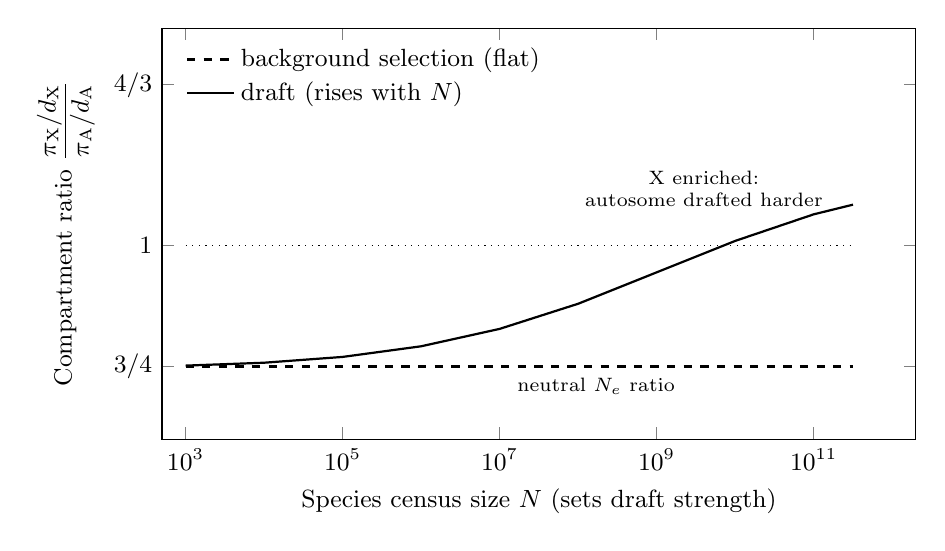
\begin{tikzpicture}
\begin{axis}[
  width=0.92\textwidth, height=6.8cm,
  xlabel={Species census size $N$ (sets draft strength)},
  ylabel={Compartment ratio $\dfrac{\pi_{\mathrm X}/d_{\mathrm X}}{\pi_{\mathrm A}/d_{\mathrm A}}$},
  xmin=2.7, xmax=12.3, ymin=0.6, ymax=1.45,
  xtick={3,5,7,9,11}, xticklabels={$10^{3}$,$10^{5}$,$10^{7}$,$10^{9}$,$10^{11}$},
  ytick={0.75,1.0,1.333}, yticklabels={$3/4$,$1$,$4/3$},
  tick label style={font=\small}, label style={font=\small},
  legend style={font=\small, at={(0.02,0.98)}, anchor=north west, draw=none, fill=none},
  legend cell align=left, clip=true, axis on top,
]
\addplot[thick, dashed, domain=3:11.5, samples=2]{0.75};
\addlegendentry{background selection (flat)}
\addplot[thick] coordinates {
(3,0.752)(4,0.758)(5,0.770)(6,0.792)(7,0.828)(8,0.880)(9,0.945)(10,1.010)(11,1.065)(11.5,1.085)};
\addlegendentry{draft (rises with $N$)}
\addplot[dotted, domain=3:11.5, samples=2]{1.0};
\node[font=\scriptsize, anchor=west] at (axis cs:7.1,0.71) {neutral $\Ne$ ratio};
\node[font=\scriptsize, anchor=south, align=center] at (axis cs:9.6,1.06) {X enriched:\\ autosome drafted harder};
\end{axis}
\end{tikzpicture}
\caption{The discriminating prediction (schematic). The within-genome X/A ratio of $\pi/d$ is pinned at the neutral effective-size ratio $3/4$ under background selection (dashed), because a size-independent reduction cancels. Under draft (solid) the ratio departs upward and grows with population size, because the larger autosome is eroded by sweeps more than the X, bounded above by $4/3$ (equation~\ref{eq:draftratio}). The steepness of the rise encodes how the adaptive substitution rate scales with population size---the quantity we know least well---so the curve's shape is illustrative, but its \emph{direction} and \emph{monotonicity} are the test. A single species samples one point on the horizontal axis; the cross-species design of \S\ref{sec:nested} reads the slope.}
\label{fig:prediction}
\end{figure}

Two features of equation~\eqref{eq:inequality} deserve emphasis. First, the prediction is bounded: draft cannot push the ratio above $4/3$ in this model, so the test lives in a narrow window, and measuring within it demands many loci and care with sampling error. Second, the prediction is about \emph{direction}, not magnitude. The curve's steepness depends on how the adaptive substitution rate scales with population size---the open quantity flagged in the companion analysis---but its sign does not. Background selection forbids any departure above $3/4$; draft forbids any departure below it. The inequality is robust even where the curve's height is not.

\subsection{Why divergence, and not raw diversity, is non-negotiable}

It is worth pausing on why the ratio of $\pi$ to $d$, rather than $\pi$ itself, is what makes the within-genome contrast work, because the point is easy to mislay. The X and an autosome differ in mutation rate. Male-biased mutation, the larger number of germline divisions in the male line, lowers the per-generation rate on the X, which spends less of its history in males. A raw comparison of $\pi_{\mathrm X}$ to $\pi_{\mathrm A}$ would read this mutational difference as though it were an effective-size difference, and the test would collapse. Equation~\eqref{eq:core} immunises against this exactly because the same male-biased rate that lowers $\pi_{\mathrm X}$ also lowers $d_{\mathrm X}$, by the same factor, and the factor cancels. The single most damaging confound of the cross-species programme---variation in $\mu$---is here neutralised by arithmetic rather than by assumption. This is the affirmative case for the design, and it is strong: short lever notwithstanding, no other test removes the mutation-rate confound so cleanly.

\section{Proposed tests, with their critiques attached}

I set out four designs of increasing ambition. Each buys back some control that the previous one lacked, and each carries a critique that the next is built to address. The honest accounting is that no single design is decisive; their value is cumulative and, in the last case, structural.

\subsection{Design 1 --- the bare transplant}

The simplest realisation uses a retrogene: a sequence reverse-transcribed from an mRNA and inserted elsewhere in the genome, frequently moving off or onto the X. One measures $\pi/d$ at the relocated copy and at its still-resident parent, and reads equation~\eqref{eq:core}.

\textbf{Critique.} Three faults make the bare transplant untrustworthy on its own. The relocated copy lands in a new local environment whose recombination rate and density of linked functional sites set its $B$, so a difference in $\pi/d$ may report a difference in local $B$ between two genomic neighbourhoods rather than the effective-size contrast we seek; the reduction $B$ is a property of the insertion site, not of the compartment. The copy is typically released from purifying constraint as it pseudogenises, inflating tolerated polymorphism and biasing the readout in the anti-draft direction, which makes the test conservative but blunt. And relocated copies that persist long enough to study are a selected sample, since insertions that established may have done so because they were useful. The bare transplant is a proof of concept, not an instrument.

\subsection{Design 2 --- the environment-matched transplant}

The first fault is the one we can engineer away. Restrict the comparison to relocated copies whose insertion site \emph{matches} the parent's in local recombination rate and in the density and selective profile of nearby functional sites, both now measurable genome-wide. With the local environment matched, $B$ is equalised across the pair by construction, and equation~\eqref{eq:core} reduces to the effective-size ratio modulated only by whatever residual scaling draft imposes---precisely the estimand of equation~\eqref{eq:inequality}.

\textbf{Critique.} Matching the environment defuses the insertion-site confound but exposes a subtler one: once $B$ is matched and constraint is controlled by restricting to demonstrably neutral sites, the homology of the transplant has done little work beyond supplying a matched starting composition, and the design converges on a standard compartment diversity-ratio comparison conditioned on local features. That is not a defect so much as a clarification---it tells us the transplant's romance is mostly rhetorical, and that the real instrument is a conditioned compartment contrast. It also leaves the deepest confound untouched: faster-X. Selection is more efficient on the hemizygous X, which depresses $\pi_{\mathrm X}/d_{\mathrm X}$ for reasons orthogonal to effective size and in the \emph{same} direction that background selection predicts, masking a draft signal if one is present.

\subsection{Design 3 --- the crossed design}

Nature performs the transplant many times and in both directions, and that redundancy is a resource. Different genes relocate into the same compartment; the same gene's homologs sit in different compartments across the genome. Treat gene identity and compartment as crossed factors and fit $\log(\pi/d)$ as their sum plus local-environment covariates,
\begin{equation}
    \log\!\big(\pi_{gi}/d_{gi}\big) \;=\; \alpha + \beta_g + \gamma_i + \delta^{\!\top}\!\mathbf{z}_{gi} + \varepsilon_{gi},
    \label{eq:mixed}
\end{equation}
where $\beta_g$ absorbs gene-specific mutational and constraint idiosyncrasies, $\gamma_i$ is the compartment effect we want, $\mathbf{z}_{gi}$ holds the local recombination rate and selected-site density, and $g$ and $i$ index gene and compartment. The compartment contrast $\gamma_{\mathrm X} - \gamma_{\mathrm A}$, estimated with gene effects and local environment partialled out, is the within-genome readout of equation~\eqref{eq:core} averaged over many natural replicates---far more robust than any single pair.

\textbf{Critique.} The crossed design tames sampling noise and per-gene idiosyncrasy, but it cannot manufacture a confound it does not measure. Faster-X still loads onto $\gamma_{\mathrm X}$, because hemizygous selection efficacy is a property of the compartment, exactly where the estimator places it. A negative or null $\gamma_{\mathrm X} - \gamma_{\mathrm A}$ is therefore uninterpretable in a single species: it could mean no draft, or it could mean draft masked by faster-X. We need a lever that moves the draft term while holding the faster-X term still.

\subsection{Design 4 --- the nested cross-species contrast}
\label{sec:nested}

Here is the resolution, and it is the design I would stake the programme on. Faster-X is a structural property of hemizygous inheritance, so to first order it is the \emph{same across species} that share the sex-determination system: it contributes a roughly constant offset to the X/A ratio regardless of how large the species is. Draft, by contrast, scales with population size. So measure the compartment contrast of equation~\eqref{eq:core} not in one species but across many spanning a range of census sizes, and ask whether the contrast \emph{changes} with species size. Background selection predicts a flat relationship at the faster-X-shifted level; draft predicts that the X's relative enrichment grows with species size, because the autosome is drafted ever harder while the X lags by its fixed three-quarters (Figure~\ref{fig:prediction}). The estimand is the slope
\begin{equation}
    \frac{\partial}{\partial \log N}\!\left[\,\frac{\pi_{\mathrm X}/d_{\mathrm X}}{\pi_{\mathrm A}/d_{\mathrm A}}\,\right]
    \;\begin{cases} = 0 & \text{background selection,}\\ > 0 & \text{draft.}\end{cases}
    \label{eq:slopeofratio}
\end{equation}
The structure of this argument is a satisfying recursion. The companion analysis dissolved the paradox by refusing to read it as a level and reading it instead as a slope; here the same move is made one level higher. Faster-X depresses the \emph{level} of the compartment ratio---an intercept effect, like background selection in the original problem---while draft tilts its \emph{slope} against species size. By differencing across species we discard the intercept, faster-X with it, and recover the slope that the mechanism actually predicts. The within-genome lever was never going to be long enough to span the paradox; nested inside the cross-species axis, it does not have to be. It supplies a $\Ne$ contrast that is \emph{internal} to each genome and therefore free of the inter-specific $\mu$ confound, while the cross-species axis supplies the range that converts a contaminated level into a clean slope.

\textbf{Critique.} The design is strong but not invulnerable, and three reservations must travel with it. Faster-X is only approximately species-invariant: if the dominance of beneficial mutations or the fraction of adaptive substitutions itself covaries with population size, part of the slope in equation~\eqref{eq:slopeofratio} is faster-X masquerading as draft, and the two cannot be separated by this design alone. Species census size is the very quantity the original paradox shows we measure poorly, so the horizontal axis carries its own error. And the cross-species axis reintroduces, in muted form, the phylogenetic non-independence and demographic heterogeneity that the within-genome retreat was meant to escape, so the regression must be phylogenetically controlled and read as suggestive of direction rather than as a point estimate of magnitude. The design buys the cleanest available test of \emph{scaling direction}; it does not buy a measurement of the paradox.

\subsection{The simulation anchor}

No empirical claim from equation~\eqref{eq:core} can be trusted until the predictions of equations~\eqref{eq:bgsratio}--\eqref{eq:draftratio} have been recovered in forward simulation, because the test is only as good as the premise that $\pi/d$ isolates $NB$ with $\mu$ and $T$ divided out. A SLiM protocol does this in three matched environments---a focal neutral window placed in an X-sized compartment, an autosome-sized compartment with quiet flanks, and an autosome-sized compartment under recurrent sweeps---and checks three things in order. The neutral substitution rate in the focal window must remain $\mu$ regardless of the linked-selection regime, confirming the Birky--Walsh premise on which the divergence ruler stands; this is the indispensable checkpoint, because it is what licenses using observed $d$ as a stand-in for $\mu$. The background-selection arm must return the ratio $3/4$ to within sampling error, recovering equation~\eqref{eq:bgsratio} and so demonstrating that a size-independent reduction truly cancels. And the draft arm must return a ratio above $3/4$ that climbs as the simulated population grows, recovering equation~\eqref{eq:draftratio}. Only after the simulation reproduces the known background-selection result and the bounded draft result can a measured departure from $3/4$ in real data be read as evidence about scaling rather than as an artefact of the estimator.

\section{What the programme can and cannot establish}

\begin{table}[h!]
\centering
\small
\caption{The four designs, by what each controls and what it leaves exposed. Control accumulates down the table; the last design alone separates draft from faster-X, and only as a direction, not a magnitude.}
\label{tab:designs}
\begin{tabular}{p{2.8cm} p{3.4cm} p{3.0cm} p{4.0cm}}
\toprule
\textbf{Design} & \textbf{Controls} & \textbf{Estimand} & \textbf{Residual confound} \\
\midrule
1. Bare transplant & $\mu$, $T$ (via $\pi/d$) & $N_iB_i/N_jB_j$ for one pair & Local $B$, relaxed constraint, biased sample. \\
\addlinespace
2. Matched environment & adds local $B$, constraint & Compartment ratio at matched $B$ & Faster-X; homology now doing little work. \\
\addlinespace
3. Crossed design & adds gene effects, sampling noise & $\gamma_{\mathrm X}-\gamma_{\mathrm A}$ over many replicates & Faster-X (loads on the compartment effect). \\
\addlinespace
4. Nested cross-species & adds the faster-X offset & $\partial(\text{ratio})/\partial\log N$ & $N$-covarying dominance; census-size error; phylogeny. \\
\bottomrule
\end{tabular}
\end{table}

The boundaries are firm and worth stating without hedging. The within-genome programme can establish that linked selection \emph{acts}, which the recombination--diversity correlation already shows, and it can establish in which \emph{direction} the reduction scales with effective size---flat for background selection, rising for draft---which is the mechanistic core of the paradox. It does this while dividing out the mutation rate exactly, the confound that most compromises the cross-species slope. What it cannot do is reproduce the \emph{magnitude} of the compression, because a fourfold effective-size lever cannot span a twelve-order-of-magnitude phenomenon however cleanly it is read. The transplant and its descendants are a mechanistic probe, sharp on direction and silent on scale, and they are most valuable not as a replacement for the cross-species regression but as its complement: the regression measures how much diversity fails to scale, and the within-genome contrast asks whether the mechanism responsible scales the way draft says it should. Lewontin's question was about the relationship between the number of organisms and the variation they carry. The within-genome transplant cannot answer it at full scale, but it can interrogate, with the mutational confound stripped away, the one thing that relationship turns on: whether linked selection bites harder the more organisms there are.

\begin{thebibliography}{99}

\bibitem{birkywalsh1988} Birky, C.W. \& Walsh, J.B. (1988). Effects of linkage on rates of molecular evolution. \emph{Proceedings of the National Academy of Sciences} 85:6414--6418.

\bibitem{buffalo2021} Buffalo, V. (2021). Quantifying the relationship between genetic diversity and population size suggests natural selection cannot explain Lewontin's paradox. \emph{eLife} 10:e67509.

\bibitem{ccc1987} Charlesworth, B., Coyne, J.A. \& Barton, N.H. (1987). The relative rates of evolution of sex chromosomes and autosomes. \emph{The American Naturalist} 130:113--146.

\bibitem{ccc1993} Charlesworth, B., Morgan, M.T. \& Charlesworth, D. (1993). The effect of deleterious mutations on neutral molecular variation. \emph{Genetics} 134:1289--1303.

\bibitem{charlesworth2009} Charlesworth, B. (2009). Effective population size and patterns of molecular evolution and variation. \emph{Nature Reviews Genetics} 10:195--205.

\bibitem{corbettdetig2015} Corbett-Detig, R.B., Hartl, D.L. \& Sackton, T.B. (2015). Natural selection constrains neutral diversity across a wide range of species. \emph{PLOS Biology} 13:e1002112.

\bibitem{elyashiv2016} Elyashiv, E., Sattath, S., Hu, T.T., et al. (2016). A genomic map of the effects of linked selection in \emph{Drosophila}. \emph{PLOS Genetics} 12:e1006130.

\bibitem{gillespie2000} Gillespie, J.H. (2000). Genetic drift in an infinite population: the pseudohitchhiking model. \emph{Genetics} 155:909--919.

\bibitem{hka1987} Hudson, R.R., Kreitman, M. \& Aguad\'e, M. (1987). A test of neutral molecular evolution based on nucleotide data. \emph{Genetics} 116:153--159.

\bibitem{leffler2012} Leffler, E.M., Bullaughey, K., Matute, D.R., et al. (2012). Revisiting an old riddle: what determines genetic diversity levels within species? \emph{PLOS Biology} 10:e1001388.

\bibitem{msh1974} Maynard Smith, J. \& Haigh, J. (1974). The hitch-hiking effect of a favourable gene. \emph{Genetical Research} 23:23--35.

\bibitem{nordborg1996} Nordborg, M., Charlesworth, B. \& Charlesworth, D. (1996). The effect of recombination on background selection. \emph{Genetical Research} 67:159--174.

\bibitem{vicoso2006} Vicoso, B. \& Charlesworth, B. (2006). Evolution on the X chromosome: unusual patterns and processes. \emph{Nature Reviews Genetics} 7:645--653.

\end{thebibliography}

\end{document}
